\documentclass[11pt]{article}
\usepackage[margin=2.2cm]{geometry}
\usepackage{booktabs}
\usepackage{amsmath,amssymb}
\usepackage{xcolor}
\usepackage{graphicx}

\definecolor{wingreen}{RGB}{0,120,60}
\definecolor{wallred}{RGB}{180,0,0}

\title{\textbf{Memoryless MAC Channels --- Results}\\[4pt]
\large Neural Polar Decoders for Two-User MAC}
\author{}
\date{April 2026}

\begin{document}
\maketitle
\thispagestyle{empty}

%% ============================================================
\section{BEMAC Class C (Corner Rate)}

$Z = X + Y$, \; $Z \in \{0,1,2\}$ (deterministic).\\
Path: \texttt{make\_path(N, N)}, $R_U \approx 0.30$, $R_V \approx 0.60$.\\
Decoder: NCG (d=16, h=64).

\begin{table}[h]\centering\small
\begin{tabular}{@{}r r r r r r@{}}
\toprule
$N$ & $k_u / k_v$ & SC & NCG & \textbf{NCG/SC} & CW \\
\midrule
  8 & 2 / 5    & 0.110 & \textbf{0.039} & \textbf{0.36$\times$} & 3K \\
 16 & 5 / 10   & 0.092 & \textbf{0.016} & \textbf{0.18$\times$} & 3K \\
 32 & 10 / 19  & 0.099 & \textbf{0.006} & \textbf{0.06$\times$} & 3K \\
 64 & 19 / 38  & 0.055 & \textbf{0.002} & \textbf{0.03$\times$} & 3K \\
128 & 38 / 77  & 0.025 & \textbf{0.0003} & \textbf{0.01$\times$} & 20K \\
256 & 77 / 154 & 0.013 & \textbf{0.0002} & \textbf{0.01$\times$} & 50K \\
512 & 154/307 & 0.003 & \textbf{0.0002} & \textbf{0.06$\times$} & 50K \\
1024 & 307/614 & 0.0004 & \textbf{0.0002} & 0.42$\times$ & 64K \\
\bottomrule
\end{tabular}
\end{table}

\begin{figure}[h]\centering
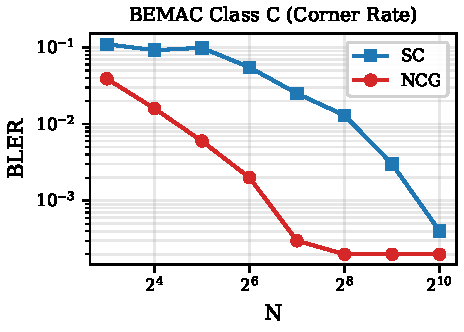
\includegraphics[width=0.75\textwidth]{plot_bemac_C.pdf}
\end{figure}

%% ============================================================
\section{BEMAC Class B (Symmetric Rate)}

$Z = X + Y$. Path: \texttt{make\_path(N, N/2)}, $R_U \approx 0.50$, $R_V \approx 0.70$.\\
Decoder: NCG (d=16, h=64).

\begin{table}[h]\centering\small
\begin{tabular}{@{}r r r r r r@{}}
\toprule
$N$ & $k_u / k_v$ & SC & NCG & \textbf{NCG/SC} & CW \\
\midrule
 16 & 8 / 11 & 0.011 & 0.011 & 1.08$\times$ & 5K \\
 32 & 16 / 22 & 0.0097 & \textbf{0.0076} & \textbf{0.78$\times$} & 15K \\
 64 & 32 / 44 & 0.0032 & 0.0032 & 1.00$\times$ & 40--48K \\
128 & 64 / 89 & 0.0014 & 0.0017 & 1.21$\times$ & 50--90K \\
256 & 128/178 & $8{\times}10^{-5}$ & $4{\times}10^{-5}$ & 0.50$\times$ & 50K \\
512 & 256/358 & 0.0 & 0.0 & --- & 2K \\
1024 & 512/716 & $10^{-4}$ & $10^{-4}$ & 1.00$\times$ & 10K \\
\bottomrule
\end{tabular}
\end{table}

\begin{figure}[h]\centering
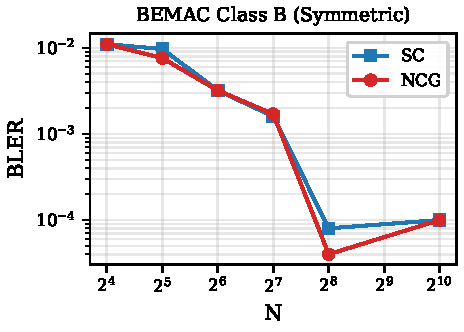
\includegraphics[width=0.75\textwidth]{plot_bemac_B.pdf}
\end{figure}

%% ============================================================
\section{GMAC Class C (Corner Rate)}

$Z = (1{-}2X) + (1{-}2Y) + W$, \; $W \sim \mathcal{N}(0, \sigma^2)$, SNR $= 6$\,dB.\\
Path: \texttt{make\_path(N, N)}, $R_U \approx 0.23$, $R_V \approx 0.45$.\\
NPD/NCG use MI-designed frozen sets (co-adapted with the neural decoder).

\begin{table}[h]\centering\small
\begin{tabular}{@{}r r r r r r r@{}}
\toprule
$N$ & $k_u / k_v$ & SC & NPD & \textbf{NPD/SC} & NCG & CW \\
\midrule
 16 &  4 / 7  & 0.162 & \textbf{0.107} & \textbf{0.66$\times$} & 0.119 & 10K \\
 32 &  7 / 15 & 0.068 & \textbf{0.037} & \textbf{0.55$\times$} & 0.035 & 10K \\
 64 & 15 / 29 & 0.027 & \textbf{0.010} & \textbf{0.37$\times$} & 0.013 & 10K \\
128 & 30 / 58 & 0.007 & 0.033 & 4.7$\times$ & \textbf{0.001} & 10--20K \\
256 & 59/117 & 0.001 & 3$\times 10^{-4}$ & 0.27$\times^*$ & --- & 20--50K \\
512 & 119/233 & 4$\times 10^{-4}$ & 2$\times 10^{-4}$ & 0.50$\times^*$ & --- & 50K \\
\bottomrule
\end{tabular}\\[3pt]
{\footnotesize $^*$N=256: 6 errors/20K CW. N=512: 11 errors/50K CW. Both unreliable.}
\end{table}

\begin{figure}[h]\centering
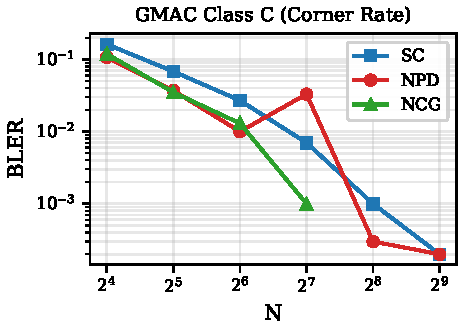
\includegraphics[width=0.75\textwidth]{plot_gmac_C.pdf}
\end{figure}

%% ============================================================
\section{GMAC Class B (Symmetric Rate)}

$Z = (1{-}2X) + (1{-}2Y) + W$, SNR $= 6$\,dB.\\
Path: \texttt{make\_path(N, N/2)}, $R_U = R_V \approx 0.48$.\\
Decoder: NCG (d=16, h=64, sequential training).

\begin{table}[h]\centering\small
\begin{tabular}{@{}r r r r r r@{}}
\toprule
$N$ & $k_u{=}k_v$ & SC & NCG & \textbf{NCG/SC} & CW \\
\midrule
 32 & 15 & 0.045 & 0.050 & 1.12$\times$ & 3K \\
 64 & 31 & 0.028 & 0.028 & 1.02$\times$ & 5K \\
128 & 62 & 0.019 & 0.023 & 1.23$\times$ & 6K \\
256 & 123 & 0.005 & \textcolor{wallred}{0.023} & \textcolor{wallred}{\textbf{4.9$\times$}} & 5--35K \\
512 & 246 & ${\sim}$0.001 & 0.012 & 12$\times$ & 10K \\
1024 & 491 & --- & 0.470 & \textcolor{wallred}{BROKEN} & 2K \\
\bottomrule
\end{tabular}
\end{table}

\begin{figure}[h]\centering
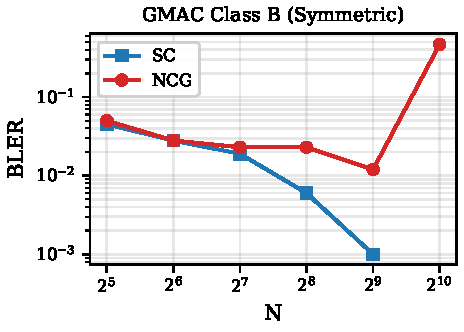
\includegraphics[width=0.75\textwidth]{plot_gmac_B.pdf}
\end{figure}

%% ============================================================
\section{ABNMAC Class B (Symmetric Rate)}

$Z = (X \oplus E_x,\; Y \oplus E_y)$, correlated binary noise.\\
Path: \texttt{make\_path(N, N/2)}, $R_U = R_V \approx 0.30$.\\
Decoder: NCG (d=16, h=64).

\begin{table}[h]\centering\small
\begin{tabular}{@{}r r r r r r@{}}
\toprule
$N$ & $k_u{=}k_v$ & SC & NCG & \textbf{NCG/SC} & CW \\
\midrule
  8 &  3 & 0.120 & 0.120 & 1.00$\times$ & 10K \\
 16 &  5 & 0.063 & \textbf{0.057} & \textbf{0.91$\times$} & 10K \\
 32 & 10 & 0.021 & \textbf{0.018} & \textbf{0.85$\times$} & 10K \\
 64 & 22 & 0.044 & \textbf{0.042} & 0.95$\times$ & 5K \\
128 & 45 & 0.029 & 0.025 & 0.87$\times$ & 4K \\
\bottomrule
\end{tabular}
\end{table}

\begin{figure}[h]\centering
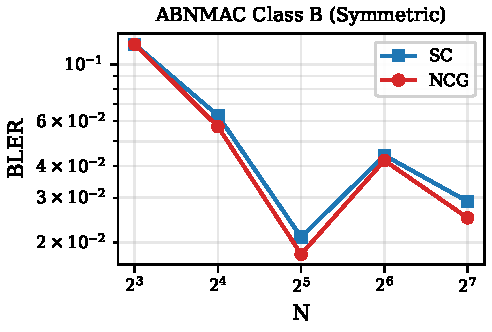
\includegraphics[width=0.75\textwidth]{plot_abnmac_B.pdf}
\end{figure}

\end{document}
